\section{引言}
\subsection{测试目标与对象}
测试面向 CLI、Qt 6 GUI、共享核心和远端服务，目标包括备份与恢复内容一致性、元数据恢复、输入拒绝、增量依赖、安全传输和失败清理。成功既要检查返回状态，也要检查磁盘内容；拒绝场景还应检查未发布部分目标和未误删既有数据。

测试采用单元、集成、系统和安装检查相结合的方法；完整测试记录和发行包补测分别列出。

\subsection{当前版本与测试结果}
测试对象为发行版本 \Code{v0.2.1-rc4}。完整功能回归在
\Code{0af622f} 上通过，包含75个构建、功能及质量检查套件入口；最终产品
\Code{0c07045} 保留该功能验证结果，并对后续打包改动执行受影响测试。
GitHub Actions 在后续合并提交 \Code{68b3cc23} 上通过。\E{E01,E15}

\begin{longtable}{L{.22\linewidth}L{.37\linewidth}L{.32\linewidth}}
\caption{最终版本及发行验证记录}\label{tab:final-validation}\\\toprule 验证项 & 实际结果 & 版本与环境\\\midrule\endfirsthead
\toprule 验证项 & 实际结果 & 版本与环境\\\midrule\endhead
功能回归 & 75/75 套件入口退出0；其中增量加密套件249/249项检查通过，覆盖三种打包格式及不加密、AES、DES 组合。 & \Code{0af622f}；RC4 保留的功能回归记录。\\
GitHub Actions & 7/7 jobs 成功：版本检查、Debian 12 构建与功能测试、客户端构建、服务端构建、Ubuntu 22.04 客户端兼容、VM systemd 验证、制品及干净容器安装。 & PR \#36 合并提交 \Code{68b3cc23}；run \Code{43165206803}。\\
RC4 产品包 & CLI 与服务器管理38/38、AppImage 自动化765/765、网络89/89、便携安装10/10项检查通过。 & 最终产品提交 \Code{0c07045}；发行包运行验收。\\
桌面 GUI & 7/7项补测通过，覆盖文件与目录选择、错误口令、证书异常和端口不可达。 & 最终 AppImage；Ubuntu 桌面。\\
归档元数据 & MyPack、USTAR、Fast-USTAR 三种格式各自完成备份恢复；共42项检查通过，核对文件内容、名称、权限、时间、链接和硬链接关系。 & 最终产品提交 \Code{0c07045}；未覆盖特权设备节点。\\
打包与安装 & deb 升级与重装各14/14项，共28/28项检查通过，涵盖数据、身份与配置保留。ZIP 解压后，命令行与服务器管理、文件元数据、公网 ECS、GUI 启动四组运行检查均通过。 & 一次性 PRoot 安装环境；原生 systemd 另由 Actions 的 VM 任务检查。\\
公开 ECS & 15条命令及29项业务检查通过，包含注册、登录、完整/增量备份、恢复、下载、删除和账户清理；合成账户已删除。归档未启用归档级 AES 加密，传输使用 BPSEC2 加密信道。 & 最终产品提交 \Code{0c07045}；Ubuntu VM 连接阿里云 ECS。\\
ECS 升级后服务 & 9项服务身份检查通过；systemd 显示 active/running，运行二进制摘要与发行包相符，监听端口及受信且有效的服务器证书均核对通过。 & 正式 ECS 实例；升级后服务核验。\\
\bottomrule\end{longtable}


\subsection{开发阶段的测试记录}
10月7日的功能回归记录为279项通过、0项失败，GUI 检查692项通过；49个构建与测试入口均退出0。后续 PR \#34 验证包含52个构建与检查入口、11个核心套件的1581条断言，以及修复后393项故障注入检查。\E{E05,E07}

数据库结构检查通过提取建表语句并在内存 SQLite 中执行，核对三张表、两个显式索引、用户外键及无视图的结构。\E{E09}

\section{功能测试}
\subsection{模块划分与判定方式}
测试分为本地备份恢复、规则与元数据、归档和编码、自动化与增量、GUI与网络、恢复安全六组。单元层检查模块状态与返回值；集成层走实际产品入口并比较文件树；网络回环测试启动服务端进程，通过 TCP 请求检查 SQLite 数据库及快照文件；GUI 层在 offscreen 环境中检查控制器与控件树，桌面操作结果见“图形界面补测”。

功能测试主要采用黑盒方法：从用户输入、归档输出和恢复结果判定行为。按等价类选择普通文件、空文件、空目录、非法路径及损坏归档；用边界值覆盖零长度、USTAR 字段容量和事件合并时间窗口；以完整备份、增量恢复及远端传输作为场景测试。预览与备份使用同一输入和规则，比较条目集合；归档与恢复通过文件树、逐字节内容、SHA-256 及元数据核对。\E{E05,E13}

每条用例列出输入与操作、预期结果、实际结果和判定。A-TC 为报告用例编号，FR 对应需求编号。A-TC-01至32中，硬链接检查（14）、Zstandard（17）及 USTAR 增量（25）依据11月记录 E15，其余依据10月功能回归 E05；A-TC-33至42依据恢复与清理修复记录 E07。\E{E05,E07,E15}

\clearpage
\subsection{代表性测试用例}
表\ref{tab:test-1}至表\ref{tab:test-6}列出42条代表性用例，覆盖正常、边界与失败输入。用例按模块分组，涵盖数据输入、编码存储、恢复输出及异常处理；Zstandard 与 USTAR 增量用例采用后续版本的运行记录。
\begingroup
\normalsize
\setlength{\tabcolsep}{4pt}
\renewcommand{\arraystretch}{1.16}
\begin{longtable}{@{}L{.14\linewidth}L{.36\linewidth}L{.21\linewidth}L{.23\linewidth}@{}}
\caption{本地备份恢复测试用例}\label{tab:test-1}\\
\toprule 用例 / 需求 & 输入、条件与操作 & 预期结果 & 实际结果与判定\\\midrule\endfirsthead
\toprule 用例 / 需求 & 输入、条件与操作 & 预期结果 & 实际结果与判定\\\midrule\endhead
\bottomrule\endfoot
\textbf{A-TC-01}\par{\footnotesize FR-101/102} & 隔离源和仓库；归档与目标不存在；普通文本及2 MiB随机binary.bin。按scripts/test.sh夹具备份、恢复，执行diff、cmp和sha256比对 & 树结构和所有文件内容一致，二进制摘要一致。 & 恢复树与源树一致，二进制文件逐字节及摘要比较通过。\par\textbf{通过}\\\addlinespace[2pt]
\textbf{A-TC-02}\par{\footnotesize FR-101/102} & 已准备仅含空文件的输入目录；empty.txt，0字节。备份恢复后检查文件存在且长度为0 & 空文件仍为空，不能遗漏或混为目录。 & 恢复后文件存在，长度为0。\par\textbf{通过}\\\addlinespace[2pt]
\textbf{A-TC-03}\par{\footnotesize FR-101/102} & 输入有空子目录；目标不存在；empty-dir/不含任何子项。备份恢复后检查该目录及其内容 & 空目录存在且仍为空。 & 恢复后空子目录存在，目录中无条目。\par\textbf{通过}\\\addlinespace[2pt]
\textbf{A-TC-04}\par{\footnotesize FR-101/102} & Linux UTF-8环境和多级目录；中文目录/带 空格.txt及嵌套文件。执行往返；按精确名称逐项检查 & 路径名、层级和字节保留。 & 恢复后的中文、空格路径及嵌套文件内容一致。\par\textbf{通过}\\\addlinespace[2pt]
\textbf{A-TC-05}\par{\footnotesize FR-101} & 仓库可写；不存在源路径；不存在的source目录。调用产品backup，记录退出码、诊断及仓库变化 & 业务失败，说明源不存在，无伪成功归档。 & 返回失败并报告源路径不存在，未生成归档。\par\textbf{通过}\\\addlinespace[2pt]
\textbf{A-TC-06}\par{\footnotesize FR-104} & 使用archive\_cli夹具隔离拓扑；archive路径位于source子树内。向夹具提供危险路径；检查源和产物 & 明确拒绝源内归档，不重复扫描输出文件。 & 拒绝源目录内的归档路径，未生成循环读取的产物。\par\textbf{通过}\\\addlinespace[2pt]
\textbf{A-TC-07}\par{\footnotesize FR-104} & 有效归档；目标已含keep.txt哨兵；非空恢复目标。执行restore，比较哨兵及目标树 & 拒绝覆盖，既有非空内容保持。 & 拒绝非空目标，keep.txt及原目标内容保持不变。\par\textbf{通过}\\\addlinespace[2pt]
\textbf{A-TC-08}\par{\footnotesize FR-103/104} & 隔离仓库；仓库外有哨兵；文件名../outside.bak。调用Resolve/Delete，比较仓库外哨兵 & 名称校验失败，不能访问或删除仓库外对象。 & 拒绝越界名称，仓库外哨兵文件内容保持不变。\par\textbf{通过}\\\addlinespace[2pt]
\end{longtable}

\begin{longtable}{@{}L{.14\linewidth}L{.36\linewidth}L{.21\linewidth}L{.23\linewidth}@{}}
\caption{规则与元数据测试用例}\label{tab:test-2}\\
\toprule 用例 / 需求 & 输入、条件与操作 & 预期结果 & 实际结果与判定\\\midrule\endfirsthead
\toprule 用例 / 需求 & 输入、条件与操作 & 预期结果 & 实际结果与判定\\\midrule\endhead
\bottomrule\endfoot
\textbf{A-TC-09}\par{\footnotesize FR-110} & a.cpp与b.txt均存在；include ext:cpp；exclude name:a.cpp。应用规则，恢复后枚举最终集合 & exclude覆盖include，a.cpp不进入归档。 & 恢复结果不含a.cpp，排除规则优先。\par\textbf{通过}\\\addlinespace[2pt]
\textbf{A-TC-10}\par{\footnotesize FR-110} & 混合.cpp、.txt、.bin输入；两个include分别为ext:cpp与ext:txt。执行筛选备份并枚举条目 & 多个include按OR，前两类进入，.bin不进入。 & .cpp和.txt文件进入归档，.bin文件被排除。\par\textbf{通过}\\\addlinespace[2pt]
\textbf{A-TC-11}\par{\footnotesize FR-111} & 同一源树和同一规则；无过滤规则的预览数据集。先preview再实际backup，比较条目集合和状态变化 & 预览集合等于真实条目；预览自身不写仓库或任务状态。 & 预览与备份条目集合一致，预览未修改仓库和任务状态。\par\textbf{通过}\\\addlinespace[2pt]
\textbf{A-TC-12}\par{\footnotesize FR-105} & 测试夹具可构造只读目录并按用例收尾；只读目录及其child文件。按metadata夹具备份恢复，检查child与目录模式 & 目录内文件可恢复；不因过早设置只读位漏掉子项。 & 子文件恢复完整，最终目录权限与原始权限一致。\par\textbf{通过}\\\addlinespace[2pt]
\textbf{A-TC-13}\par{\footnotesize FR-201} & 支持POSIX软链接的隔离目录；link指向一个既有文件。按USTAR单元测试往返，用lstat/readlink验证 & 恢复为软链接且目标文本一致，不复制为普通文件。 & lstat识别为符号链接，readlink读出的目标文本一致。\par\textbf{通过}\\\addlinespace[2pt]
\textbf{A-TC-14}\par{\footnotesize FR-201} & 在同一文件系统内创建两个指向同一inode的文件路径；分别用MyPack、USTAR和Fast USTAR备份恢复，核对内容及硬链接关系。 & 恢复后的两个路径共享inode，文件内容一致。 & 恢复后的两个路径指向同一inode，文件内容一致。\par\textbf{通过}\\\addlinespace[2pt]
\end{longtable}

\begin{longtable}{@{}L{.14\linewidth}L{.36\linewidth}L{.21\linewidth}L{.23\linewidth}@{}}
\caption{归档与编码测试用例}\label{tab:test-3}\\
\toprule 用例 / 需求 & 输入、条件与操作 & 预期结果 & 实际结果与判定\\\midrule\endfirsthead
\toprule 用例 / 需求 & 输入、条件与操作 & 预期结果 & 实际结果与判定\\\midrule\endhead
\bottomrule\endfoot
\textbf{A-TC-15}\par{\footnotesize FR-120} & 构造合法普通文件及超界链接名；超出USTAR linkname容量的链接目标。调用USTAR编码并检查错误 & 明确拒绝无法表达字段，不截断生成错误归档。 & 编码返回失败并给出字段限制原因，未生成截断归档。\par\textbf{通过}\\\addlinespace[2pt]
\textbf{A-TC-16}\par{\footnotesize FR-121} & 编译compression单元程序；单一重复字节组成的缓冲区。Huffman编码后解码并逐字节比较 & 单符号输入可往返，解码长度和字节一致。 & 单符号输入成功往返，解码长度与字节一致。\par\textbf{通过}\\\addlinespace[2pt]
\textbf{A-TC-17}\par{\footnotesize FR-121} & 使用标准 Zstd 工具及项目编解码器，输入随机、重复、边界长度、损坏与截断数据；执行双向互操作并比较恢复内容。 & 支持范围内的标准流正确解码，内容一致；损坏、截断及未支持扩展被拒绝，失败不发布输出。 & 标准工具互操作及内容比较通过；损坏、截断和未支持的扩展被拒绝，原输出保持不变。\par\textbf{通过}\\\addlinespace[2pt]
\textbf{A-TC-18}\par{\footnotesize FR-122/123} & 手动完整MyPack，交互口令或测试注入；AES-256-CTR-HMAC，固定测试目录和非空测试口令。生成容器，再以正确口令恢复并比较树 & 认证与恢复成功，归档不保存明文口令。 & 正确口令下认证及恢复通过，恢复树与输入一致。\par\textbf{通过}\\\addlinespace[2pt]
\textbf{A-TC-19}\par{\footnotesize FR-122} & 已有加密容器，目标不存在；与写入时不同的恢复口令。调用恢复，记录错误并检查目标 & 认证失败，不发布部分目标，不产生可用的明文输出。 & 报告认证失败，目标未发布。\par\textbf{通过}\\\addlinespace[2pt]
\textbf{A-TC-20}\par{\footnotesize FR-122/404} & 复制有效容器，隔离原件；payload单字节翻位。对副本恢复，检查诊断与目标 & 摘要或认证检查拒绝损坏输入，不发布部分目录树。 & 损坏内容被拒绝，未发布部分恢复目录。\par\textbf{通过}\\\addlinespace[2pt]
\end{longtable}

\begin{longtable}{@{}L{.14\linewidth}L{.36\linewidth}L{.21\linewidth}L{.23\linewidth}@{}}
\caption{自动化与增量测试用例}\label{tab:test-4}\\
\toprule 用例 / 需求 & 输入、条件与操作 & 预期结果 & 实际结果与判定\\\midrule\endfirsthead
\toprule 用例 / 需求 & 输入、条件与操作 & 预期结果 & 实际结果与判定\\\midrule\endhead
\bottomrule\endfoot
\textbf{A-TC-21}\par{\footnotesize FR-140} & 任务已有有效完整基线；与基线相同的源树。到期Evaluate或立即EvaluateNow，比较前后归档数 & 报告无变化并跳过，不产生新快照；立即检查不强制生成快照。 & 报告无变化并跳过，归档数量不变。\par\textbf{通过}\\\addlinespace[2pt]
\textbf{A-TC-22}\par{\footnotesize FR-140/404} & state曾记录基线，隔离仓库；删除被绑定的基线归档，保留manifest/state。再次运行计划评估 & 不能因manifest相同跳过；重建完整基线并说明原因。 & 发现基线缺失后创建完整快照，未误判为无变化。\par\textbf{通过}\\\addlinespace[2pt]
\textbf{A-TC-23}\par{\footnotesize FR-141} & 使用注入时钟的去抖对象；窗口内连续两个事件批次。NoteEvents后检查Due，推进到静默/最大等待边界并Consume & 事件合并为一代，边界到期触发；数量为事件数。 & 窗口内事件合并，推进时钟到边界后触发一次消费。\par\textbf{通过}\\\addlinespace[2pt]
\textbf{A-TC-24}\par{\footnotesize FR-305} & 已有强manifest完整基线；同长度改写文件并还原原mtime。执行incremental backup，核对种类和变更计数 & 识别内容变化并生成delta，不按size/mtime漏检。 & 同长度、同mtime的内容修改被识别，生成增量快照。\par\textbf{通过}\\\addlinespace[2pt]
\textbf{A-TC-25}\par{\footnotesize FR-102/305} & 已有 USTAR 完整基线；修改、新增和删除文件后执行增量备份，检查快照类型和父依赖，再恢复最新快照并逐文件比较。 & 生成有效增量快照，依赖关系正确，恢复结果与源目录一致。 & 生成USTAR增量及正确父依赖，恢复后新增、修改、删除结果与源目录一致。\par\textbf{通过}\\\addlinespace[2pt]
\textbf{A-TC-26}\par{\footnotesize FR-403} & base→delta链，后代为需保留还原点；淘汰计划仅拟删除仍被引用的base。调用单项删除/保留计划，检查全部链材料 & 保护被保留后代依赖的祖先并如实计数，不能断链。 & 依赖祖先被保留，仍可恢复保留的后代快照。\par\textbf{通过}\\\addlinespace[2pt]
\end{longtable}

\begin{longtable}{@{}L{.14\linewidth}L{.36\linewidth}L{.21\linewidth}L{.23\linewidth}@{}}
\caption{GUI与网络测试用例}\label{tab:test-5}\\
\toprule 用例 / 需求 & 输入、条件与操作 & 预期结果 & 实际结果与判定\\\midrule\endfirsthead
\toprule 用例 / 需求 & 输入、条件与操作 & 预期结果 & 实际结果与判定\\\midrule\endhead
\bottomrule\endfoot
\textbf{A-TC-27}\par{\footnotesize FR-130} & Qt offscreen、独立配置与仓库；真实GUI受管备份/恢复/删除流程。执行 GUI 自检，检查控件、控制器和归档结果 & 控件正确调用核心；产物为v2，列表、恢复和删除与磁盘一致。 & 操作后界面列表、归档文件和恢复内容一致，删除结果同步。\par\textbf{通过}\\\addlinespace[2pt]
\textbf{A-TC-28}\par{\footnotesize FR-304} & 本地服务器要求BPSEC2，测试证书有效；客户端配置不受信任的离线根。发起握手，观察业务请求是否到达 & 身份验证失败，不能继续登录或退回明文。 & 握手拒绝不可信根，未进入登录阶段。\par\textbf{通过}\\\addlinespace[2pt]
\textbf{A-TC-29}\par{\footnotesize FR-304} & 服务端require\_bpsec2=true；BPSEC1 ClientHello。建立连接尝试降级握手 & 服务端拒绝BPSEC1，不接受降级业务会话。 & 服务端拒绝BPSEC1握手，未建立降级业务会话。\par\textbf{通过}\\\addlinespace[2pt]
\textbf{A-TC-30}\par{\footnotesize FR-301/302} & 两个有效账户，A已上传快照；B请求A的快照id。以B会话调用下载或删除，直接检查A的blob与元数据 & 拒绝跨账户访问，A的数据不变。 & 账户B的下载和删除请求被拒绝，账户A数据保持不变。\par\textbf{通过}\\\addlinespace[2pt]
\textbf{A-TC-31}\par{\footnotesize FR-302} & 服务端采用5次/60秒的测试配置；同名连续5次错误口令后立即给正确口令。达到阈值，再以正确口令登录并查限速记录 & 锁定窗口内正确口令同样被拒，不能靠猜中一次绕过。 & 达到阈值后正确口令仍被拒绝，锁定窗口生效。\par\textbf{通过}\\\addlinespace[2pt]
\textbf{A-TC-32}\par{\footnotesize FR-303} & 已有schema1与旧用户/快照行；追加链列中途注入失败。打开可写存储触发迁移，检查列/版本，解除注入重开 & 失败整体回滚，重试成功且旧数据保留；只读路径不升级。 & 注入失败后结构及版本回滚；解除注入后迁移成功，旧记录保留。\par\textbf{通过}\\\addlinespace[2pt]
\end{longtable}

\begin{longtable}{@{}L{.14\linewidth}L{.36\linewidth}L{.21\linewidth}L{.23\linewidth}@{}}
\caption{恢复安全测试用例}\label{tab:test-6}\\
\toprule 用例 / 需求 & 输入、条件与操作 & 预期结果 & 实际结果与判定\\\midrule\endfirsthead
\toprule 用例 / 需求 & 输入、条件与操作 & 预期结果 & 实际结果与判定\\\midrule\endhead
\bottomrule\endfoot
\textbf{A-TC-33}\par{\footnotesize FR-102/305} & 建立base、delta1、delta2；first从v1到v2，另增second，keep不变。恢复第三个还原点，与独立完整备份结果逐节点比较 & 两个delta及未改动内容都在，链恢复等于完整恢复。 & 链恢复结果与独立完整恢复结果逐节点一致。\par\textbf{通过}\\\addlinespace[2pt]
\textbf{A-TC-34}\par{\footnotesize FR-102/404} & 非特权用户，前序链成功，目录ro为0500；最后delta新增ro/new.txt，合并不可写。恢复目标链并检查目标和中间资源 & 整体失败，错误指向合并，不发布目标，只清理由本次操作创建且已核验身份的资源。 & 最后增量合并失败使整次恢复失败，未发布目标。\par\textbf{通过}\\\addlinespace[2pt]
\textbf{A-TC-35}\par{\footnotesize FR-102/404} & 三份快照有效；预置阻挡中间容器提取的对象。恢复最终还原点，检查失败和目标 & 中间提取失败传播至整次失败，不发布部分树。 & 中间容器提取失败后停止恢复，目标未发布。\par\textbf{通过}\\\addlinespace[2pt]
\textbf{A-TC-36}\par{\footnotesize FR-102/404} & 有基线与一个delta；把增量数据改为同长度垃圾。尝试链恢复，核对诊断和发布状态 & 内层或预检拒绝损坏材料，返回失败且无目标发布。 & 损坏增量被拒绝，整次恢复失败，目标未发布。\par\textbf{通过}\\\addlinespace[2pt]
\textbf{A-TC-37}\par{\footnotesize FR-102/404} & 非特权用户，基线含0500目录；delta含无法在只读父目录删除的删除标记。按测试夹具执行链恢复 & 删除标记失败使整次失败，不发布缺失删除的结果。 & 删除标记处理失败后终止恢复，未发布缺少删除操作的结果。\par\textbf{通过}\\\addlinespace[2pt]
\textbf{A-TC-38}\par{\footnotesize FR-102/404} & 有效增量链，容器位置被阻挡；error\_message参数为nullptr。调用链恢复入口并检查bool和目标 & 无诊断指针仍返回false，不误报成功或发布目标。 & 诊断指针为空时仍返回false，目标未发布。\par\textbf{通过}\\\addlinespace[2pt]
\textbf{A-TC-39}\par{\footnotesize FR-104/404} & 目标旁owner名字已是到哨兵的硬链接；同名owner硬链接及原始哨兵正文。调用恢复，检查inode、正文和目标 & 排他创建失败，不能O\_TRUNC哨兵；恢复失败且不发布。 & 排他创建失败，哨兵内容与inode不变，目标未发布。\par\textbf{通过}\\\addlinespace[2pt]
\textbf{A-TC-40}\par{\footnotesize FR-102} & 有效快照，目标多级父目录不存在；missing/a/b/restored。经产品恢复入口运行并比对结果 & 可建立缺失父目录并成功恢复，不能因提前open父目录引入回归。 & 缺失的多级父目录被创建，恢复内容比较通过。\par\textbf{通过}\\\addlinespace[2pt]
\textbf{A-TC-41}\par{\footnotesize FR-104/404} & 按专用测试进程装配LD\_PRELOAD，注入必须命中；首次增量临时目录已创建但身份查询失败。运行临时资源故障注入脚本，核对哨兵、标记、目标与汇总 & 返回失败，不删除身份无法验证的对象，保留标记与诊断，不发布目标。 & 注入命中后返回失败，未删除无法核验身份的对象，目标未发布。\par\textbf{通过}\\\addlinespace[2pt]
\textbf{A-TC-42}\par{\footnotesize FR-104/404} & 原父目录缺失，装配注入器；父目录创建后，外来目录抢占暂存目录名。专用测试进程确定性造冲突，核对外来哨兵/inode/权限 & 保留外来对象，返回失败且不发布目标。 & 外来目录及哨兵的内容、inode和权限不变，恢复返回失败。\par\textbf{通过}\\\addlinespace[2pt]
\end{longtable}

\endgroup


\subsection{测试操作与复现}
在 Linux 源码根目录构建各目标，再执行测试脚本。以下为核心复现命令，测试脚本创建独立目录并检查退出码及文件内容：
\begin{verbatim}
make -j4 all server gui-all cert-tool test-fixtures
bash scripts/incremental_encryption_test.sh
bash scripts/claim_failure_test.sh
bash scripts/final_gate.sh
\end{verbatim}
故障注入测试使用 LD\_PRELOAD，并检查注入命中和哨兵文件；需要普通用户权限的场景由专用测试进程执行。完整脚本及环境要求见仓库测试文档。\E{E05,E10,E15}

\subsection{Zstandard 与增量组合验证}
Zstandard 回归使用项目编解码器与标准 Zstd 命令行工具双向对照，输入包括空数据、边界长度、随机、重复、混合数据以及损坏和截断流。记录中29项互操作检查通过；56份标准流中38份正确解码，18份使用未支持扩展的输入被明确拒绝。2613份格式与异常输入中9份被接受并与标准工具输出比对一致，其余2604份被拒绝；既有文件、符号链接以及失败时内存输出保持不变的检查均通过。旧 LZSS+Huffman 流式往返测试继续用于格式兼容检查。\E{E15,E16}

增量加密套件的249项检查覆盖 MyPack、USTAR、Fast USTAR，以及不加密、AES、DES 和 Zstandard 组合。A-TC-25 对应其中的 USTAR 增量生成与恢复；RC4 AppImage 自动化记录还包含 USTAR 定时及实时增量的快照类型、父依赖与恢复摘要检查。\E{E15}

\subsection{测试样例与覆盖范围}
最终演示目录中的样例用于本机覆盖不同目录结构和文件类型。它们由演示目录的
\Code{tests/fixtures/generate\_fixtures.py} 生成；云端往返使用普通小目录。\E{E15}

\begin{longtable}{L{.16\linewidth}L{.39\linewidth}L{.36\linewidth}}
\caption{本机测试样例及用途}\label{tab:final-samples}\\\toprule 样例 & 内容 & 测试用途\\\midrule\endfirsthead
\toprule 样例 & 内容 & 测试用途\\\midrule\endhead
\Code{ordinary/} & 5个文件，含文本、中文文件名、带空格路径、1 KiB二进制文件和空文件；另有嵌套目录。 & 完整备份、打包/压缩/加密组合、恢复、错误口令及本地服务；云端只用此类小目录。\\
\Code{large-tree/} & 30个子目录，各含100个80字节文件；共3000个文件，数据240000字节。 & 本机检查目录遍历、文件数和进度显示。\\
\Code{special-files/} & 相对符号链接、FIFO、权限为000的文件、二进制及空文件，另含中文和空格路径。 & 检查特殊类型及不可读文件的失败行为。权限测试须以普通用户执行；root或具备 \Code{CAP\_DAC\_OVERRIDE} 的进程可绕过权限。\\
\Code{incremental/v0-v2} & v0建立基线；v1、v2分别修改、新增和删除文件，并保留未变化文件。 & 检查增量链的新增、修改、删除、未变化文件及恢复结果。\\
\Code{realtime-live/} & 配套脚本逐秒新增一个文件，连续约7秒。 & 配合实时任务检查文件事件合并及随后生成的快照。\\
\bottomrule\end{longtable}

云端验收使用专用合成账户和
\Code{ordinary/} 小目录，完成登录、完整备份、增量备份、恢复、下载及账户清理。
\E{E15}

\subsection{图形界面补测}
Ubuntu 桌面上的 AppImage 补测共7项，全部通过，覆盖文件与目录选择及五类连接错误。测试通过 X11 输入操作窗口，结合 AT-SPI 检查控件状态，并捕获窗口截图。证书异常由隔离的 SecureChannel 测试服务触发；错误口令使用本地服务器，端口不可达使用绑定但未监听的本机端口。\E{E15}

\begin{longtable}{L{.22\linewidth}L{.49\linewidth}L{.20\linewidth}}
\caption{AppImage 图形界面补测}\label{tab:rc4-gui-tests}\\\toprule 用例 & 检查结果 & 截图\\\midrule\endfirsthead
\toprule 用例 & 检查结果 & 截图\\\midrule\endhead
导入服务器身份文件 & 打开、取消、重新打开并导入身份文件；窗口正常，server\_id 自动回填。 & \figref{fig:rc4-dialog-evidence}\\
选择备份源目录 & 打开、取消、重新打开，选择子目录并确认；源路径正确回填，未意外启动备份。 & \figref{fig:rc4-dialog-evidence}\\
错误口令 & 登录被拒绝，界面提示账号信息错误，仍保持未登录状态。 & \figref{fig:rc4-auth-evidence}\\
证书已过期 & 连接终止并提示证书过期或尚未生效。 & \figref{fig:rc4-auth-evidence}\\
证书内容被改动 & 连接终止并提示服务器身份证书无效。 & \figref{fig:rc4-connection-evidence}\\
证书与身份密钥不匹配 & 连接终止并提示证书和服务器密钥不一致。 & \figref{fig:rc4-connection-evidence}\\
TCP 端口不可达 & 登录失败；界面提示连接中断且已有数据不会被覆盖。 & \figref{fig:rc4-connection-evidence}\\
\bottomrule\end{longtable}

\begin{center}
\begin{minipage}{.48\linewidth}\centering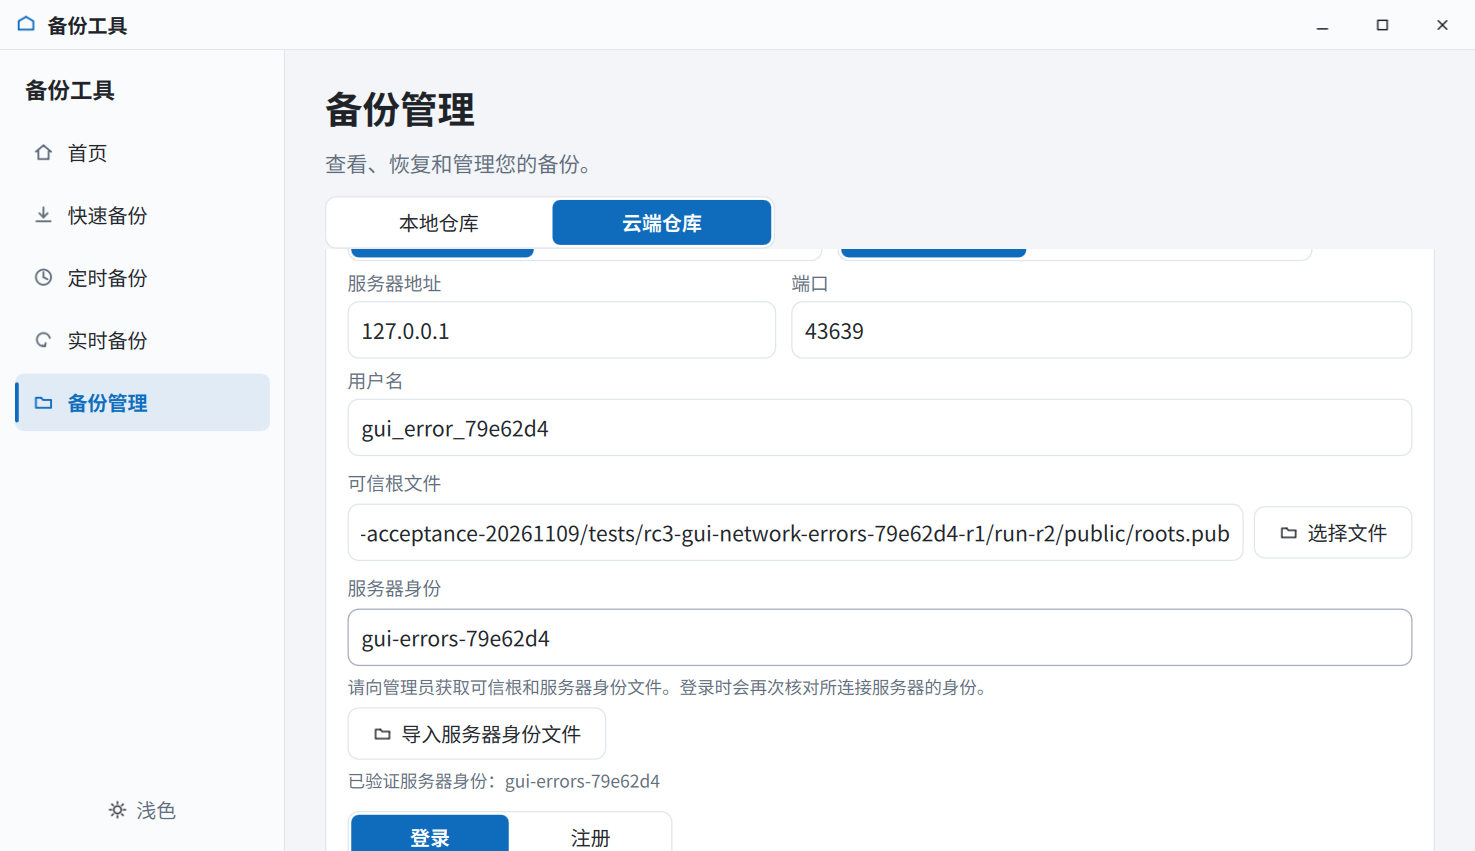
\includegraphics[width=\linewidth,height=.28\textheight,keepaspectratio]{figures/test-screenshots/rc4-file-dialog-imported.png}\par\small 导入服务器身份文件\end{minipage}\hfill
\begin{minipage}{.48\linewidth}\centering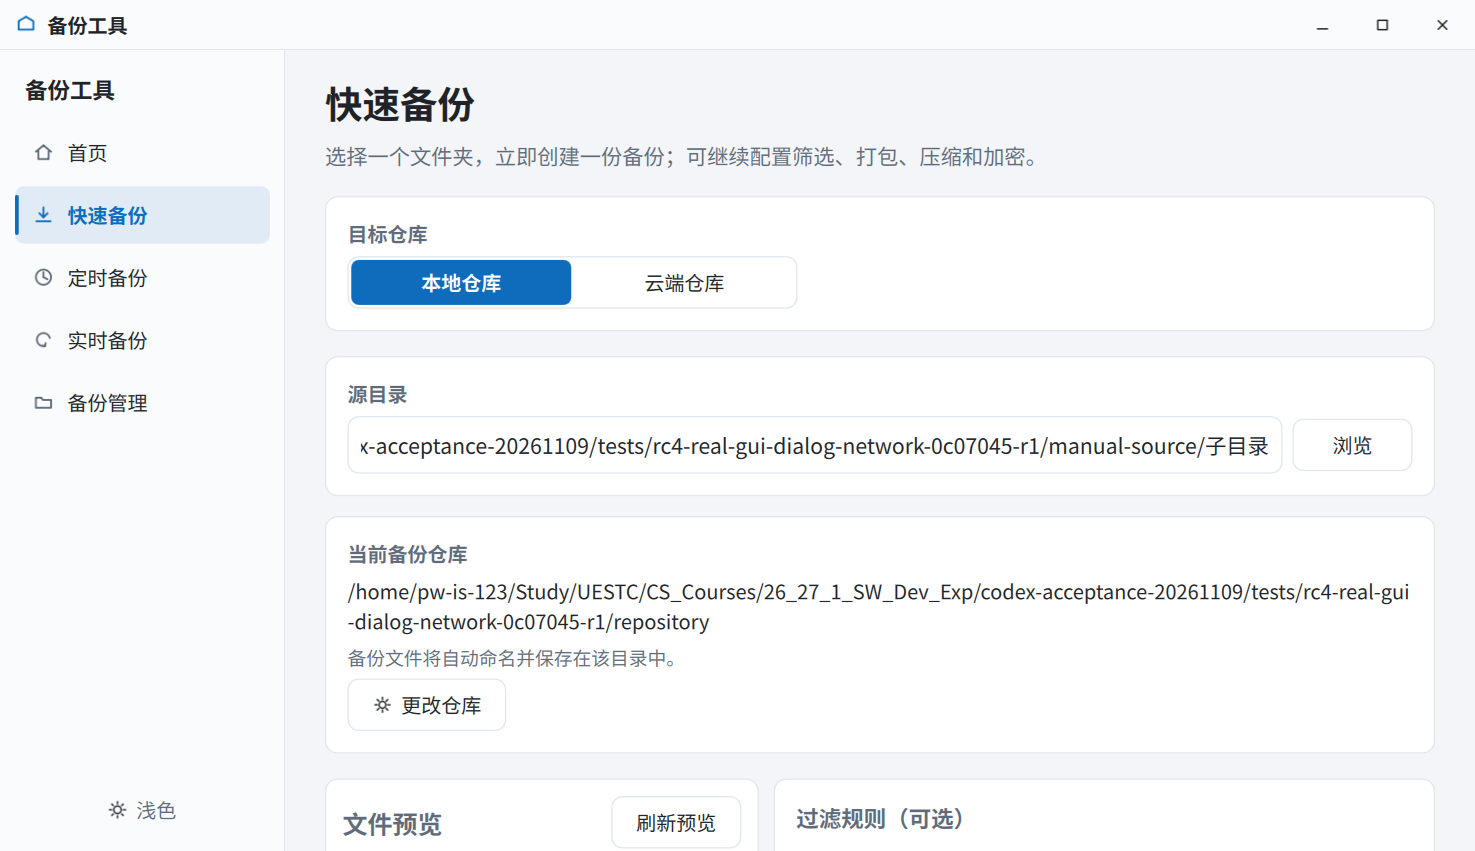
\includegraphics[width=\linewidth,height=.28\textheight,keepaspectratio]{figures/test-screenshots/rc4-folder-source-updated.png}\par\small 选择备份源目录\end{minipage}
\captionof{figure}{AppImage 的文件与目录选择补测}\label{fig:rc4-dialog-evidence}
\end{center}

\begin{center}
\begin{minipage}{.48\linewidth}\centering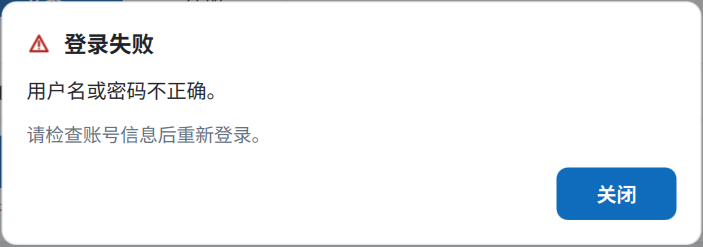
\includegraphics[width=\linewidth,keepaspectratio]{figures/test-screenshots/dialog-crops/rc4-wrong-password-crop.png}\par\small 错误口令\end{minipage}\hfill
\begin{minipage}{.48\linewidth}\centering
\includegraphics[width=\linewidth,keepaspectratio]{figures/test-screenshots/dialog-crops/rc4-expired-certificate-crop.png}\par\small 证书过期\end{minipage}
\captionof{figure}{AppImage 的认证与证书失败提示}\label{fig:rc4-auth-evidence}
\end{center}

\begin{center}
\begin{minipage}{.48\linewidth}\centering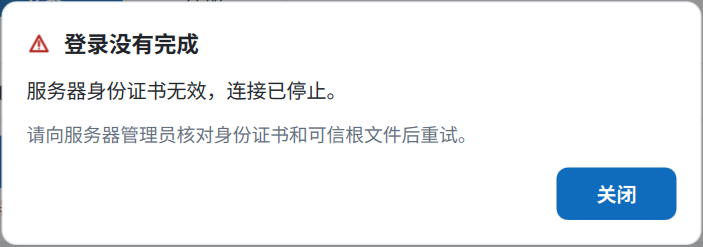
\includegraphics[width=\linewidth,keepaspectratio]{figures/test-screenshots/dialog-crops/rc4-tampered-certificate-crop.png}\par\small 证书被改动\end{minipage}\hfill
\begin{minipage}{.48\linewidth}\centering
\includegraphics[width=\linewidth,keepaspectratio]{figures/test-screenshots/dialog-crops/rc4-key-mismatch-crop.png}\par\small 证书与密钥不匹配\end{minipage}
\vspace{.5em}
\begin{minipage}{.64\linewidth}\centering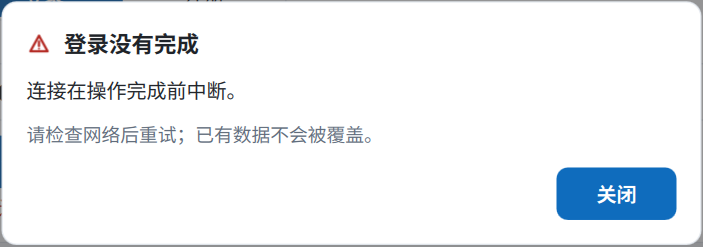
\includegraphics[width=\linewidth,keepaspectratio]{figures/test-screenshots/dialog-crops/rc4-tcp-unreachable-crop.png}\par\small 连接端口不可达\end{minipage}
\captionof{figure}{AppImage 的服务器身份与连接错误提示}\label{fig:rc4-connection-evidence}
\end{center}

\clearpage
服务器管理菜单截图来自2026年11月12日的隔离实例测试，展示本地服务端的运行状态
与身份信息，对应提交 \Code{aa49607}。\E{E15}

\begin{center}
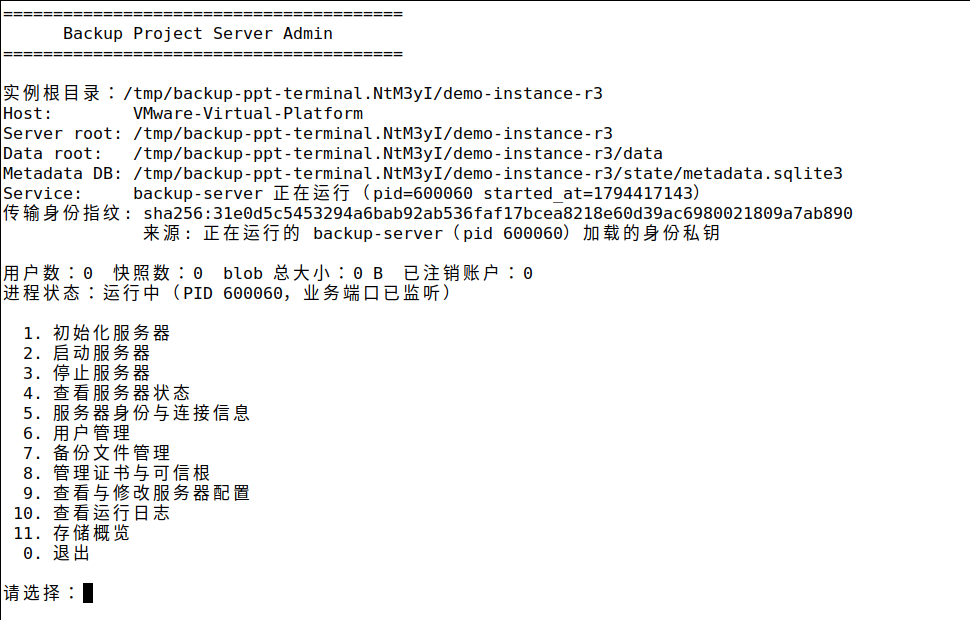
\includegraphics[width=\linewidth,keepaspectratio]{figures/test-screenshots/34-server-menu-running-crop.png}
\captionof{figure}{隔离实例中的本地服务器运行状态与身份信息}\label{fig:server-menu-evidence}
\end{center}

\subsection{界面功能展示截图}
图\ref{fig:gui-local-evidence}至图\ref{fig:gui-remote-evidence}展示本地备份、增量记录、云端备份与恢复流程，截图来自2026年11月11日的操作记录。\E{E15}

\begin{center}
\begin{minipage}{.48\linewidth}\centering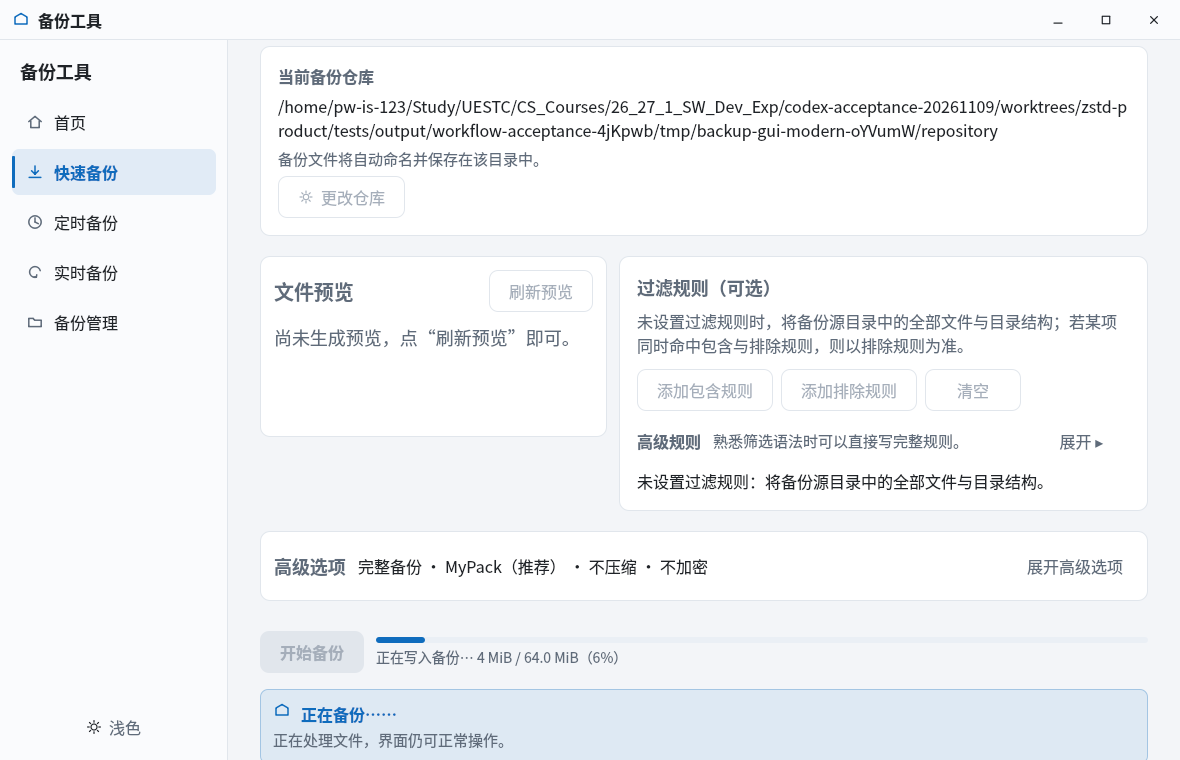
\includegraphics[width=\linewidth,height=.27\textheight,keepaspectratio]{figures/test-screenshots/08-local-backup-progress.png}\par\small 本地备份进度\end{minipage}\hfill
\begin{minipage}{.48\linewidth}\centering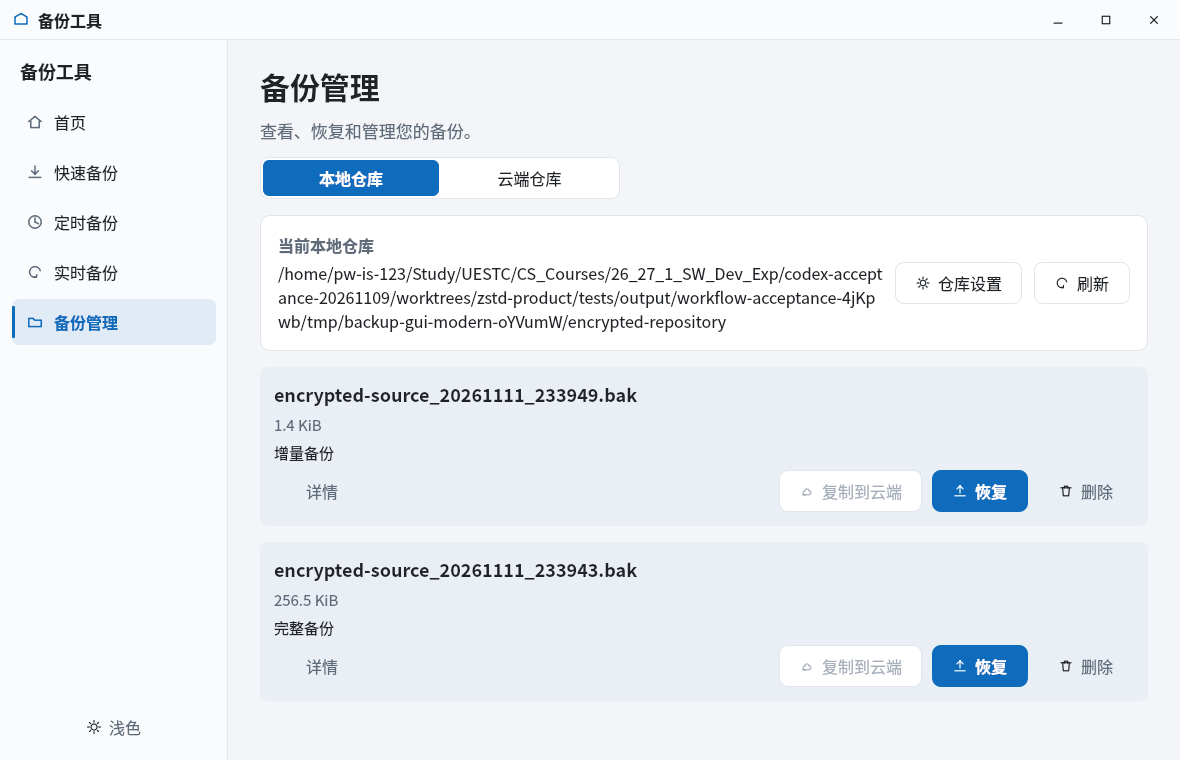
\includegraphics[width=\linewidth,height=.27\textheight,keepaspectratio]{figures/test-screenshots/09-encrypted-incremental-record.png}\par\small 加密增量记录\end{minipage}
\captionof{figure}{客户端本地备份及增量快照界面}\label{fig:gui-local-evidence}
\end{center}

\begin{center}
\begin{minipage}{.48\linewidth}\centering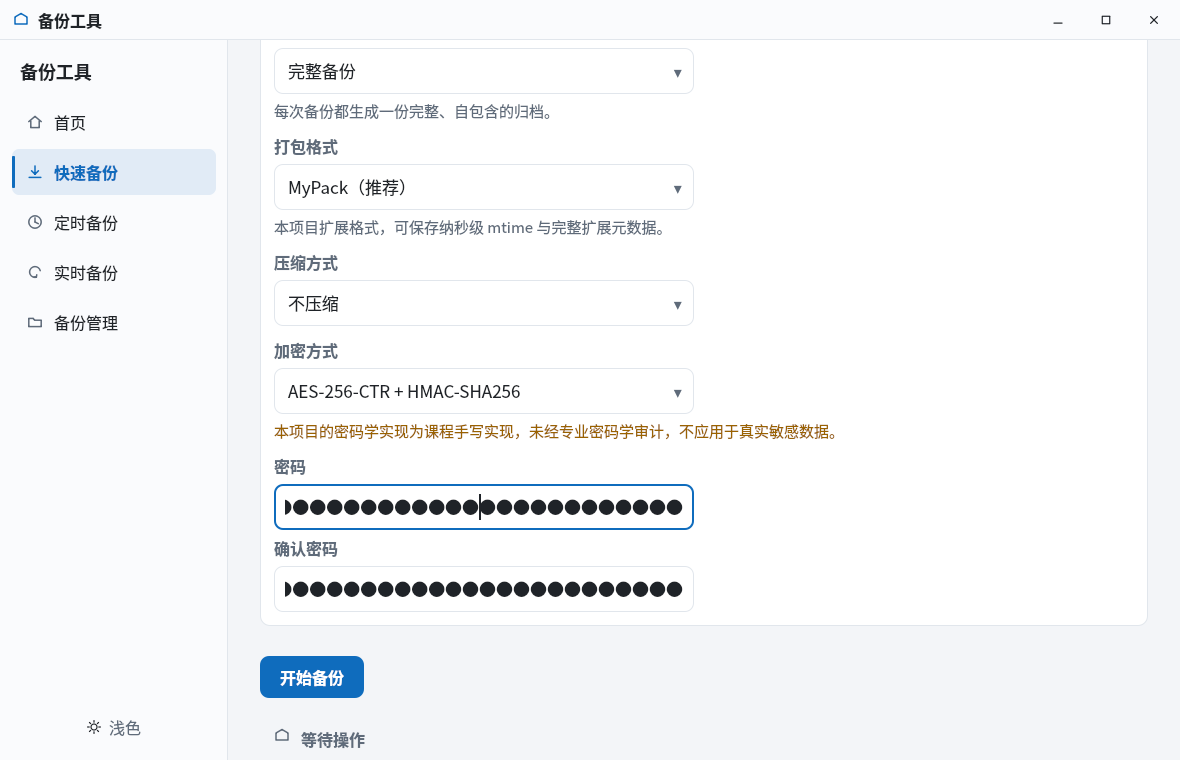
\includegraphics[width=\linewidth,height=.27\textheight,keepaspectratio]{figures/test-screenshots/10-encrypted-backup-password.png}\par\small 加密备份的口令输入\end{minipage}\hfill
\begin{minipage}{.48\linewidth}\centering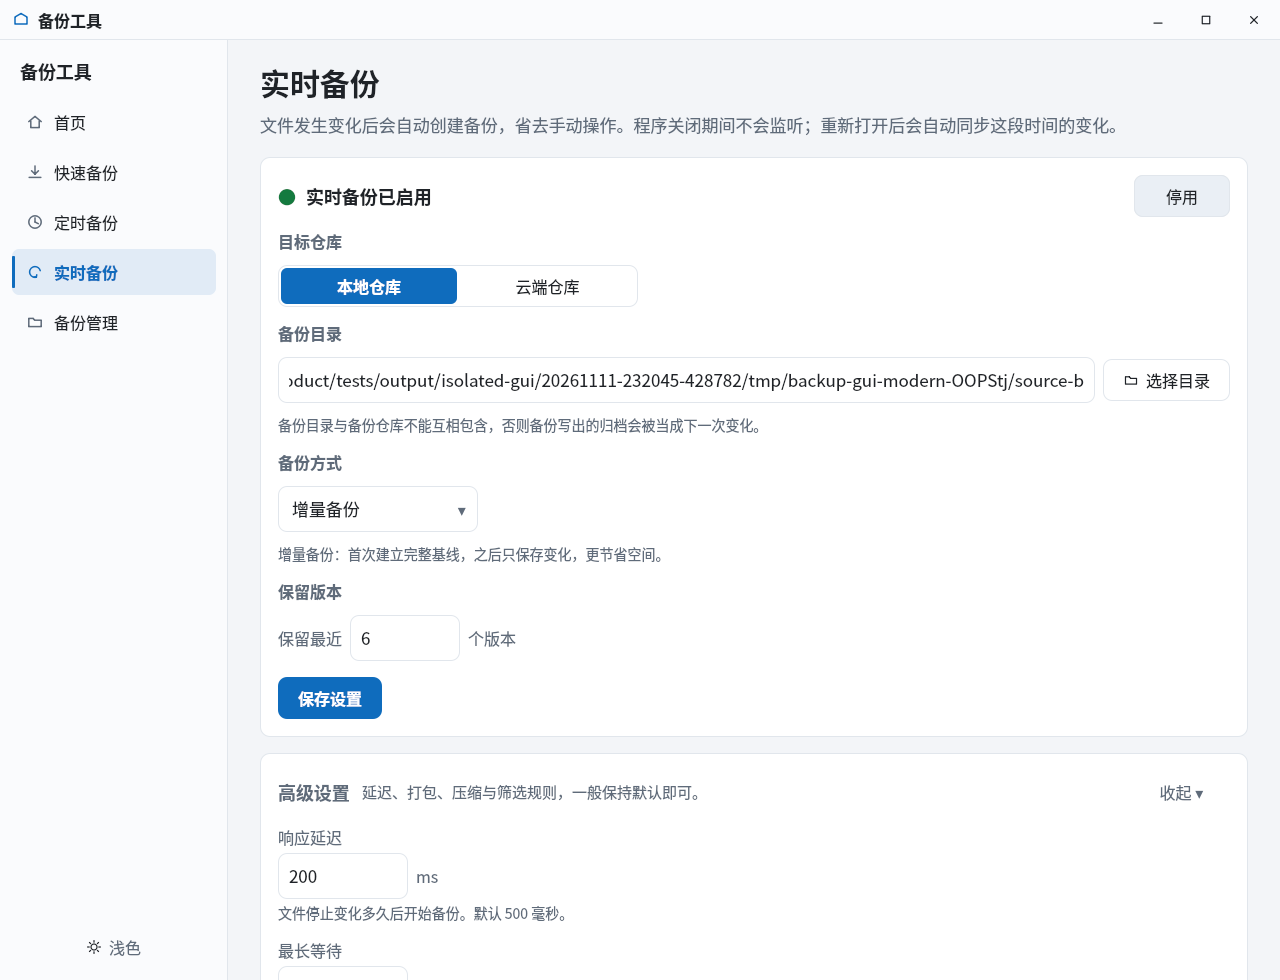
\includegraphics[width=\linewidth,height=.27\textheight,keepaspectratio]{figures/test-screenshots/04-realtime-delta.png}\par\small 实时任务生成增量快照\end{minipage}
\captionof{figure}{加密备份与实时备份界面}\label{fig:gui-automation-evidence}
\end{center}

\begin{center}
\begin{minipage}{.48\linewidth}\centering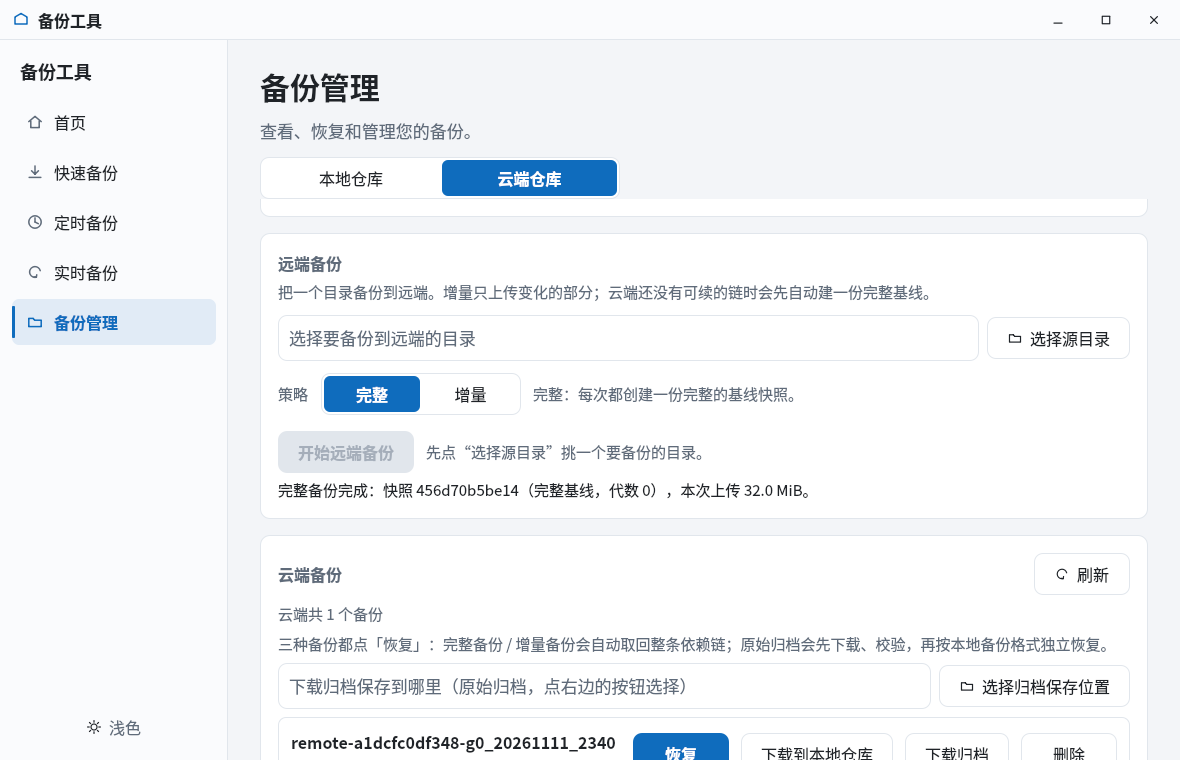
\includegraphics[width=\linewidth,height=.27\textheight,keepaspectratio]{figures/test-screenshots/22-cloud-upload-complete.png}\par\small 云端备份完成\end{minipage}\hfill
\begin{minipage}{.48\linewidth}\centering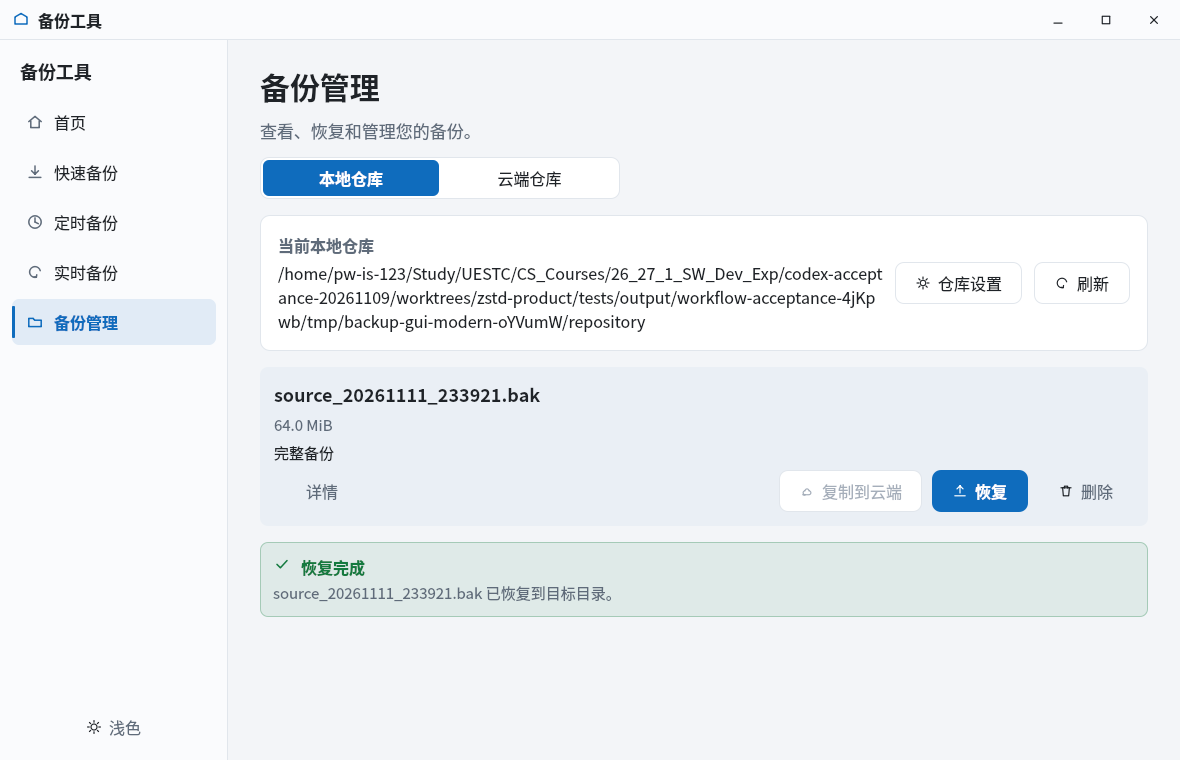
\includegraphics[width=\linewidth,height=.27\textheight,keepaspectratio]{figures/test-screenshots/24-local-restore-complete.png}\par\small 本地恢复完成\end{minipage}
\captionof{figure}{客户端云端备份和本地恢复界面}\label{fig:gui-remote-evidence}
\end{center}


\clearpage
\section{代码测试}
\subsection{静态检查与源码抽查}
源码抽查覆盖增量恢复、文件写入与清理、过滤规则和服务端存储。检查项目包括命名与格式、注释准确性、接口返回值、长度及整数类型、输入限制、文件描述符与临时目录的生命周期。增量恢复重点检查失败状态是否向上层返回，并阻止发布；配置保存重点检查短写、同步失败及替换后的返回状态。\E{E08,E10,E12}

clang-format 按 Google C++ 样式检查，ShellCheck 检查构建和测试脚本，行宽检查覆盖可处理的源码与注释。2026年10月15日的记录中，注释率为21.55\%，未发现可处理范围内超过80列的代码或注释；PR \#34 记录中的格式及 ShellCheck 检查通过。\E{E07,E08}

QML 静态检查保留了已确认的工具诊断清单：Qt 6.4.2 的 qmllint 无法完整识别由 C++ 注册的上下文属性，以及部分枚举和延迟赋值。脚本按文件、属性和诊断类别匹配这些记录，出现清单外的诊断即失败；相应界面另由运行测试检查。\E{E05,E13}

\subsection{GoogleTest 与关键分支检查}
GoogleTest 用于快照目录和过滤规则构建器：前者57个测试、8个测试组，后者22个测试、11个测试组，记录均通过。测试源码保留在 \Code{tests/unit/}；其他核心模块使用项目的断言测试程序。\E{E13,E15}

白盒测试按实现中的关键分支构造条件：过滤规则检查 include 的 OR、exclude 的优先级以及非法规则不改变原状态；增量恢复分别触发基线失败、中间增量失败、合并失败及诊断指针为空；数据库迁移在事务中途注入失败，核对回滚和重试。A-TC-09、10、32及33至42分别给出这些输入与结果。\E{E05,E07,E10}

\subsection{内存与资源检查}
Valgrind 3.22 检查 config、preview、Zstandard 备份及恢复四条 CLI 执行，使用 MyPack 打包且不启用归档加密。四次执行均正常退出，19项核对通过，未报告内存错误或确定、间接内存泄漏。对应源码为 \Code{aa49607}，图\ref{fig:valgrind-log}展示恢复场景记录。ASan/UBSan 的开发阶段记录包含41次调用，均未报告内存或未定义行为错误。\E{E15,E18}

\begin{center}
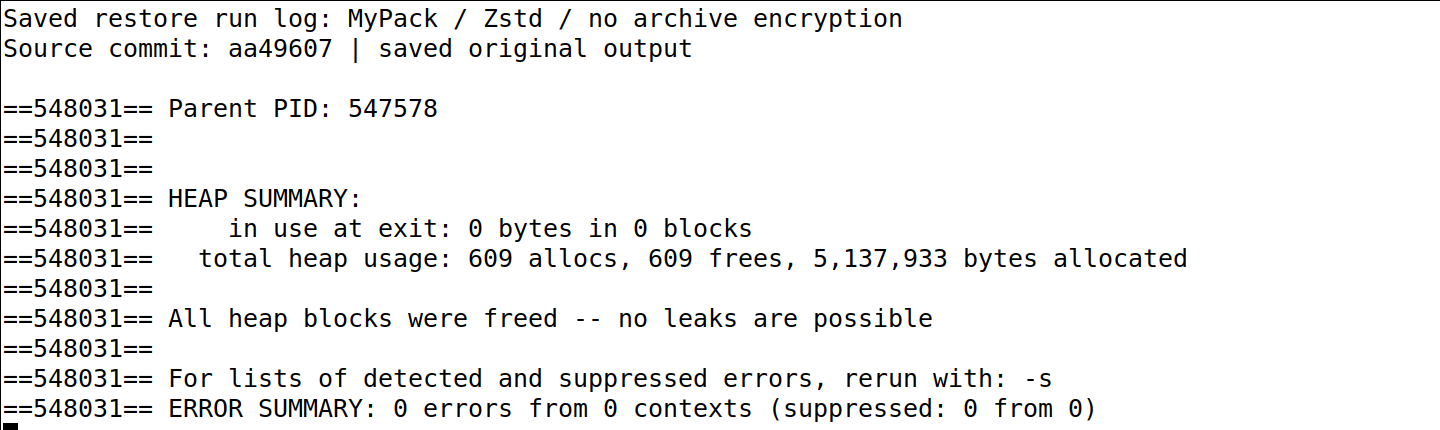
\includegraphics[width=\linewidth,height=.25\textheight,keepaspectratio]{figures/test-screenshots/37-valgrind-saved-log.png}
\captionof{figure}{Valgrind 的恢复执行记录}\label{fig:valgrind-log}
\end{center}

\section{性能测试}
\subsection{对象、环境与测量方法}
性能测试针对项目的流式 Huffman、Zstandard 及文件 I/O 模块，源码版本为 \Code{0af622f}。运行环境为 Ubuntu 虚拟机、8个 vCPU，宿主处理器为 Intel Core i7-10750H；内核版本为 \Code{7.0.0-42-generic}。编译使用 GCC、C++17、\Code{-O2 -g}，gprof 构建另加 \Code{-pg}；分析工具为 gprof 2.42 和 perf 7.0.14。\E{E18}

输入由固定种子生成，包含文本、重复、结构化、随机及混合五类数据，每类分别为64 KiB、1 MiB和4 MiB。每种输入对不压缩、Huffman和Zstandard各执行三次往返，交错运行并取中位数，共45个组合、135次往返。计时包含输出创建、编解码、同步及文件发布，内容生成和摘要计算在计时之外。每次解码后比较 SHA-256，所有比较通过。环境使用共享虚拟机，未清空文件系统缓存。\E{E18}

\subsection{压缩大小与时间}
表\ref{tab:codec-performance}列出4 MiB输入的实测结果，压缩大小包含格式头部。不压缩时输出均为4,194,304字节；编码、解码时间为三次测量的中位数，原始数据见 \Code{test-records/performance/comparison-summary.csv}。
\begin{longtable}{L{.13\linewidth}L{.15\linewidth}R{.20\linewidth}R{.18\linewidth}R{.18\linewidth}}
\caption{4 MiB输入的压缩大小与编解码时间}\label{tab:codec-performance}\\\toprule 数据 & 算法 & 压缩字节数 & 编码 / ms & 解码 / ms\\\midrule\endfirsthead
\toprule 数据 & 算法 & 压缩字节数 & 编码 / ms & 解码 / ms\\\midrule\endhead
\bottomrule\endfoot
文本 & Huffman & 2,869,817 & 57.45 & 141.54\\
文本 & Zstandard & 8,018 & 14.60 & 68.32\\
重复 & Huffman & 4,194,580 & 65.28 & 165.65\\
重复 & Zstandard & 17,298 & 16.13 & 74.06\\
结构化 & Huffman & 2,462,262 & 52.13 & 123.26\\
结构化 & Zstandard & 757,648 & 55.81 & 87.15\\
随机 & Huffman & 4,194,580 & 63.79 & 162.12\\
随机 & Zstandard & 4,194,514 & 45.50 & 54.58\\
混合 & Huffman & 3,879,214 & 65.01 & 173.82\\
混合 & Zstandard & 2,304,596 & 39.91 & 65.39\\
\end{longtable}


Zstandard 对文本和重复内容的编码结果明显更短；随机内容缺少可利用的重复，输出为4,194,514字节，略大于原输入。Huffman 对随机和该重复字节分布样例也有头部开销。混合输入中，Zstandard 输出2,304,596字节，小于Huffman的3,879,214字节，编码和解码中位时间也更短；结构化输入的两种编码时间接近，Zstandard 的解码时间更短。具体差异与数据分布有关。

\Needspace{6\baselineskip}
\subsection{函数耗时分析与大样本计时}
gprof 使用128 MiB混合流：每个64 KiB块由32 KiB重复文本和32 KiB固定伪随机字节组成。编码耗时0.782秒，解码耗时2.200秒；恢复后的 SHA-256 与原样本一致。编码采样中 \Code{Parse} 占73.33\%，\Code{Encode} 占18.33\%，\Code{HuffLiterals} 占6.67\%；解码采样中 \Code{Decode} 占99.45\%。编码优化可优先检查匹配解析过程，解码优化则集中在 \Code{Decode}。采样周期为0.01秒，编译器内联会影响函数归属。\E{E18}

同一128 MiB样本另以常规 \Code{-O2} 构建执行 \Code{perf stat -e duration_time}，编码经过时间为0.882秒，恢复摘要一致。该环境的 \Code{perf_event_paranoid=4}，cycles、instructions及task-clock事件未取得测量值。上述结果测量编解码与文件落盘，归档打包、GUI和网络传输不在本组计时内。\E{E18}

\begin{center}
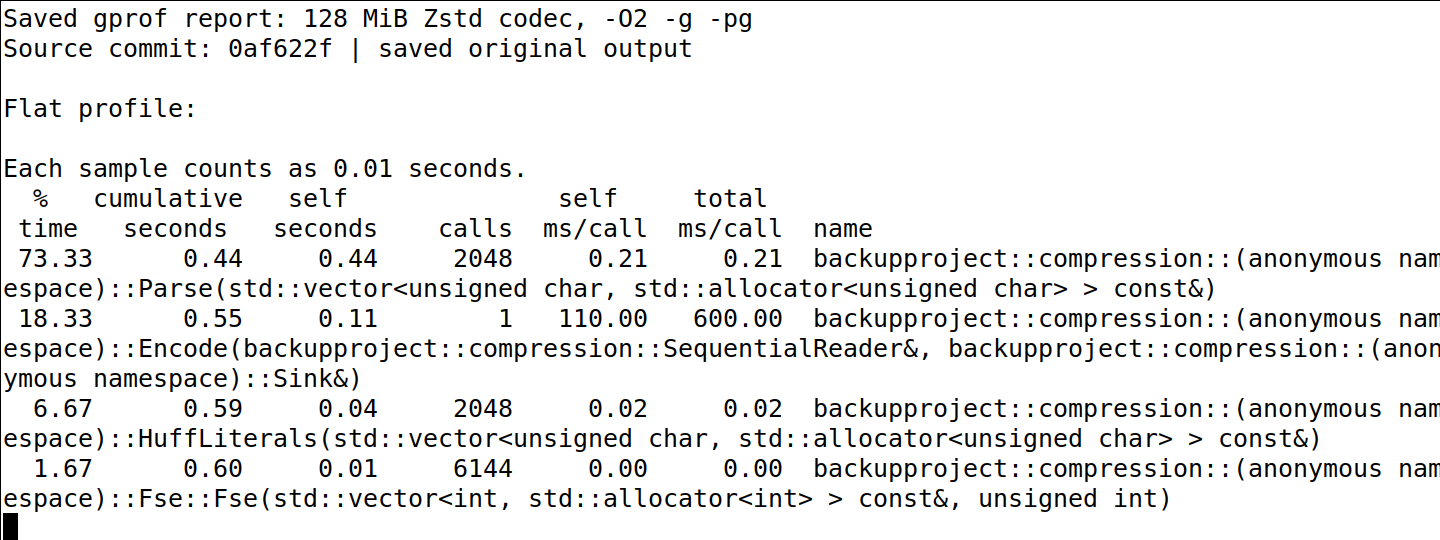
\includegraphics[width=\linewidth,height=.25\textheight,keepaspectratio]{figures/test-screenshots/38-gprof-saved-encode.png}
\captionof{figure}{128 MiB Zstandard 编码的 gprof 采样}\label{fig:gprof-log}
\end{center}
\begin{center}
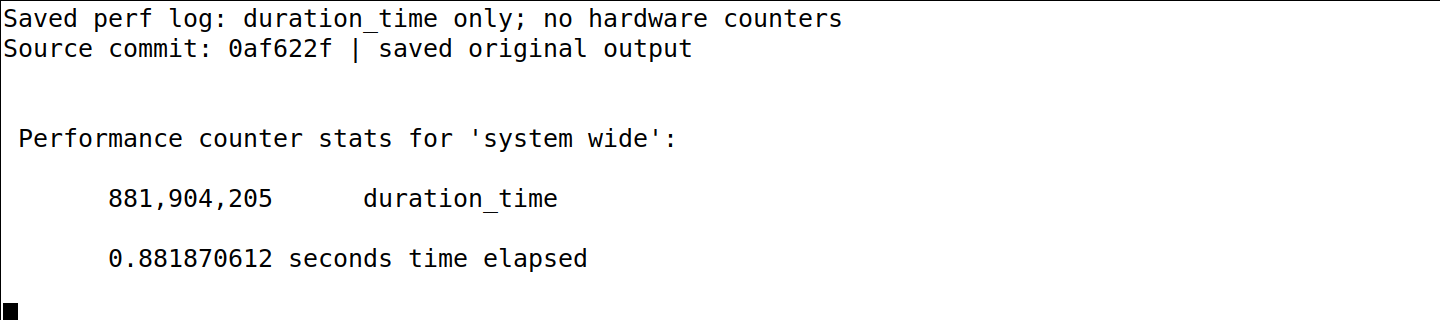
\includegraphics[width=\linewidth,height=.19\textheight,keepaspectratio]{figures/test-screenshots/39-perf-saved-duration.png}
\captionof{figure}{perf 的编码经过时间记录}\label{fig:perf-log}
\end{center}

\subsection{重复运行与资源限制}
开发阶段质量测试连续执行10轮稳定性检查，10轮均通过。归档流水线还在 \Code{RLIMIT_AS} 地址空间限制下检查流式处理，并核对输出内容和失败清理。\E{E05}

\section{健壮性测试}
\subsection{异常输入与中断处理}
对有效样本制作独立副本，再截断头部或数据流、翻转归档字节、使用错误口令、移除父快照，或提供越界路径和非空恢复目标。调用产品恢复入口，记录退出状态和错误信息，同时检查目标是否发布、既有文件是否改变。相应的 A-TC-05至08、19、20及34至39均按预期拒绝，原数据与哨兵保持不变。\E{E05,E07}

连接中断测试在上传或下载过程中断开 TCP，重新建立连接后核对续传状态与已接收数据摘要，再继续传输；数据库测试在迁移中途注入失败，检查事务回滚后能否重新打开和重试。相应网络与存储套件通过，数据库迁移的输入和结果见 A-TC-32。\E{E05,E15}

\subsection{系统调用故障与恢复目录保护}
测试程序在隔离目录放置哨兵文件，通过链接期替换或 \Code{LD\_PRELOAD} 在指定系统调用注入失败；测试记录检查注入是否命中，随后比较错误状态、文件内容、inode、权限、文件描述符关闭次数和目标发布结果。

\begin{longtable}{L{.21\linewidth}L{.35\linewidth}L{.35\linewidth}}
\caption{故障注入过程与检查结果}\label{tab:fault-results}\\\toprule 对象 & 干扰与检查步骤 & 实际结果\\\midrule\endfirsthead
\toprule 对象 & 干扰与检查步骤 & 实际结果\\\midrule\endhead
\bottomrule\endfoot
文件同步与关闭 & 使fsync返回ENOSPC、使close返回EIO；检查关闭调用次数及首个错误是否保留。 & 同步失败后仍执行关闭；错误信息保留首次失败原因，相关断言通过。\\
身份材料读取 & 在读满私钥后的一次尾部读取注入EINTR，检查重试及多余字节识别。 & 中断后重试，超长输入被拒绝；未把读取中断当作合法文件结束。\\
增量恢复 & 令中间提取、删除标记或合并失败；检查最终返回值、目标及暂存目录。 & 错误使整次恢复失败，未发布部分目标；无诊断指针时结果相同。\\
临时目录身份 & 目录创建后使身份查询失败，或让外来目录占用后续暂存名称；比较哨兵和权限。 & 保留无法核验归属及外来对象，返回失败，未发布目标。\\
\end{longtable}
以上分别对应清理、读取重试和临时资源测试。资源清理问题修复后的393项检查通过；用例 A-TC-41、42列出两种目录干扰的具体结果。\E{E05,E07}

\section{测试结果分析}
\subsection{缺陷案例}
R-01 在 PR \#30 修复，其触发条件是增量链恢复在 delta 提取、容器还原或合并等步骤失败，旧代码中的部分 break 只退出内层循环，外层发布流程仍可能继续。修复后，各失败分支设置独立的失败标志，发布前统一检查；即使调用方不接收错误文本，仍返回失败。回归包括多 delta 的完整对照、最后或中间 delta 失败、空目标和错误文本指针为空，相关定义见 INC-R T10～T15。

PR \#34 后续修复了临时资源归属确认失败时误删对象的问题。在修复前的故障注入测试中，397项检查有25项未通过。修正创建、归属核验与清理逻辑后，调整后的393项检查全部通过。\E{E07}

文件对话框在早期安装包中曾因运行依赖缺失而崩溃。补齐依赖后，最终 AppImage 通过“打开、取消、重新选择、导入”的操作检查，目录选择和五类连接错误提示也通过。该缺陷以正常桌面入口复测，并对照控件状态与窗口截图确认结果。\E{E15}

\subsection{结果汇总与结论}
\begin{longtable}{L{.21\linewidth}L{.39\linewidth}L{.31\linewidth}}
\caption{按测试类型汇总的结果}\label{tab:test-result-analysis}\\\toprule 类型与模块 & 检查内容 & 结果与分析\\\midrule\endfirsthead
\toprule 类型与模块 & 检查内容 & 结果与分析\\\midrule\endhead
\bottomrule\endfoot
功能：归档与恢复 & 普通与特殊文件、过滤、压缩加密、完整与增量、元数据和恢复依赖。 & 对应内容、摘要、元数据及失败行为检查通过，见六组用例表。\\
功能：自动任务与远端 & 定时与实时触发、无变化跳过、账户隔离、传输与续传、界面状态同步。 & 记录中的业务检查通过；文件对话框依赖问题修复后补测通过。\\
代码与内存 & 格式、注释、接口和异常分支；GoogleTest、Valgrind及ASan/UBSan。 & 格式和分支断言通过；所测执行未报告内存错误。QML工具诊断按已确认清单处理。\\
性能：编解码 & 三种规模、五类语料的重复测量，128 MiB样本的函数采样及计时。 & 往返摘要一致；压缩大小及中位时间见表\ref{tab:codec-performance}，主要编码采样耗时集中于Parse。\\
健壮性：失败恢复与清理 & 损坏归档、错误输入、系统调用失败、迁移回滚和临时目录冲突。 & 修复后相关检查通过；失败状态阻止发布，受保护的既有数据保持不变。\\
\end{longtable}
